\chapter{\IfLanguageName{dutch}{Proof of Concept}{Proof of Concept}}%
\label{ch:poc}

\section{\IfLanguageName{dutch}{Applicatie Ontwerp}{Application Design}}%
\label{sec:design}
To achieve the greatest flexibility, client-server architecture will be used. One of the biggest advantages of this solution is the ability to share information resources among different users or devices belonging to the same user. In other words, data consistency is improved, what ensures all clients access the latest data from a one central source, minimizing divergences. Moreover centralized data storage allows for effective backups and management, enhancing data reliability. There is also possibility for errors isolation - client applications failures do not affect the server or other clients, what improves overall system stability making maintanace easier.

\begin{figure}[H]
    \centering
    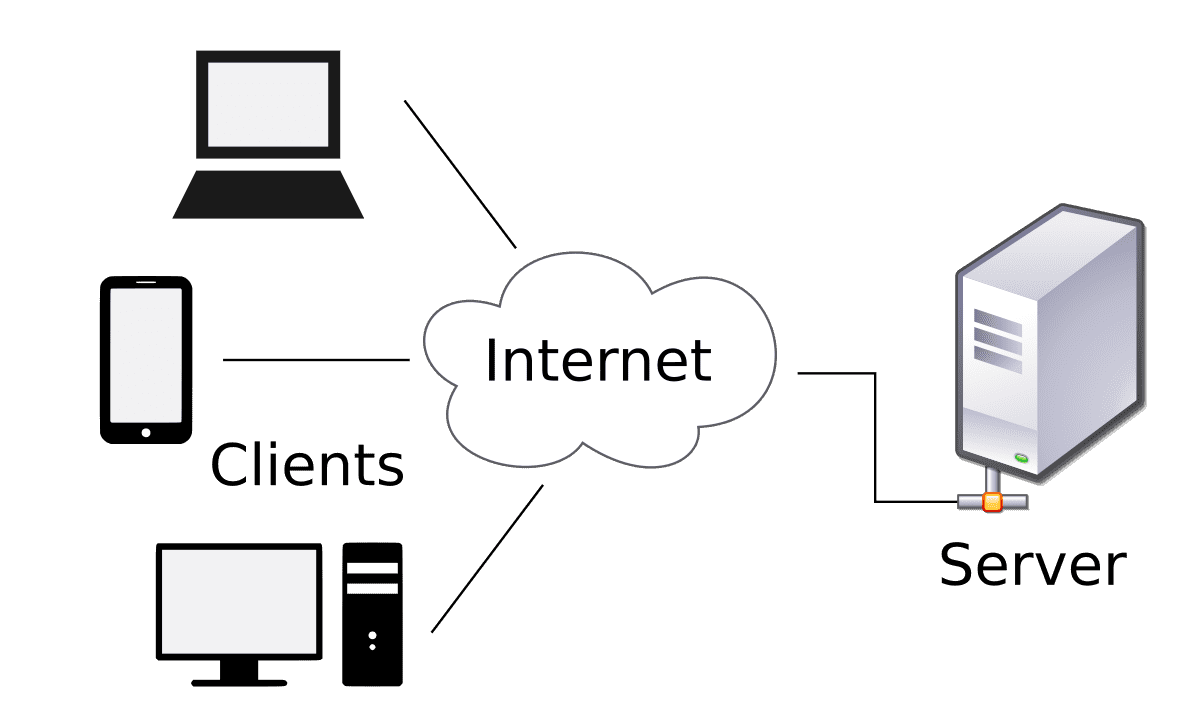
\includegraphics[width=0.8\textwidth]{client-server-architecture.png}
    \caption[Layout]{\label{fig:architecture} Solution client-server architecture }
\end{figure}

\begin{figure}[H]
    \centering
    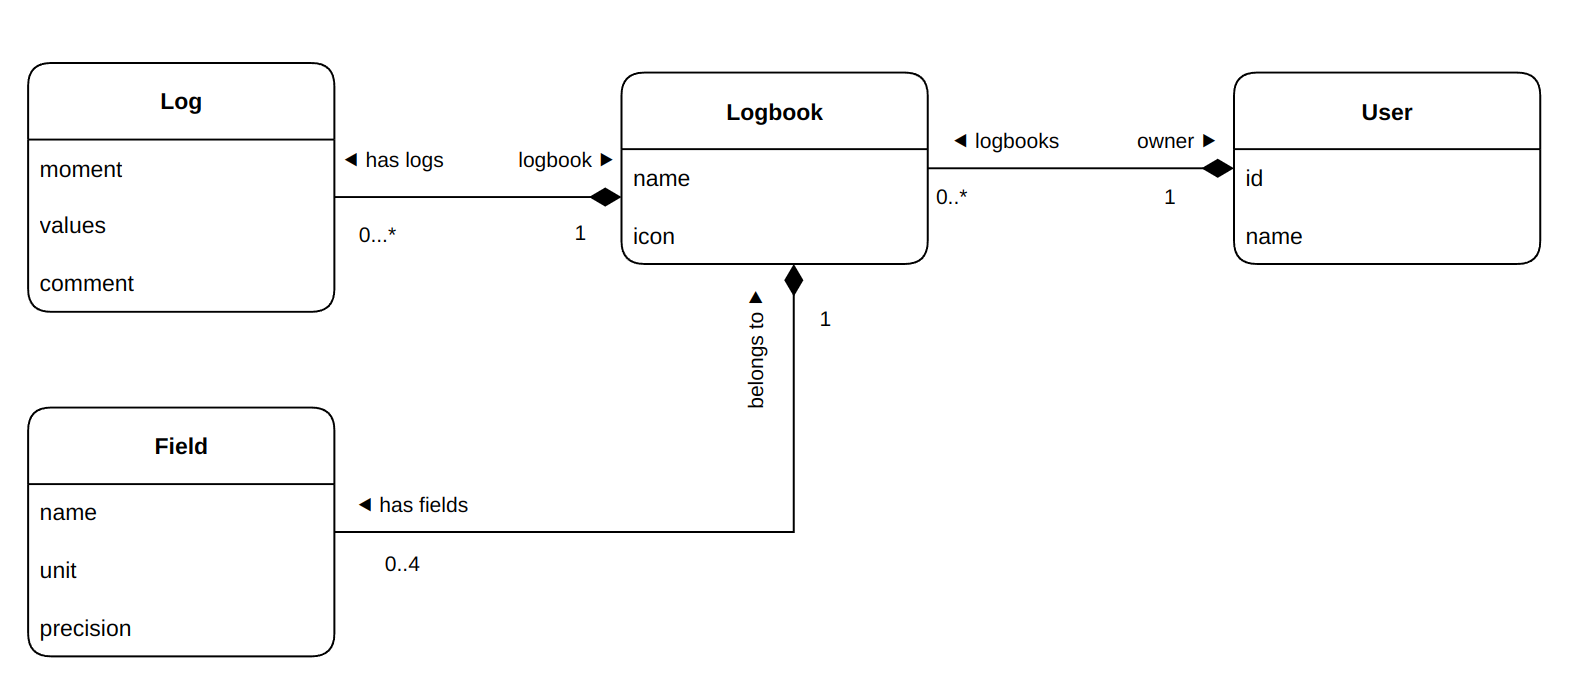
\includegraphics[width=0.9\textwidth]{conceptual-model.png}
    \caption[Layout]{\label{fig:conceptualmodel} Conceptual model diagram }
\end{figure}


\section{\IfLanguageName{dutch}{Voorbereiding}{Prerequisites}}%
\label{sec:prerequisites}

The software is being developed on a PC machine with x64 architecture running Fedora Linux. The project  will be managed on the Azure DevOps where tasks are described and issues tracked. GitHub repository was initialized for code version control and cloned locally. The machine has already installed Node.js - a JavaScript runtime environment, Node Package Manager (npm) and Node Version Manager (nvm). Detailed installation is not a subject of this thesis.

Quasar framework provides own command line interface (CLI) allowing access to more features and automating some tasks. The CLI will be installed globally to make possible to directly run Quasar commands in the terminal, run a local http server for testing or do upgrades on the project \autocite{QuasarStart}. According to the Quasar documentation, the following code needs to be executed:

\begin{verbatim}
    npm i -g @quasar/cli

\end{verbatim}

\section{\IfLanguageName{dutch}{Installatie}{Client Template Installation}}%
\label{sec:installation}

New Quasar project is initialised with the command:
\begin{verbatim}
    npm init quasar@latest

\end{verbatim}

Installation wizard asks some questions about preferences to automatically generate startup project template. The developer chooses first a project type (in most cases it's an application) and folder name. Command is executed inside already initialised git repo, so folder 'client' becomes a subfolder of the whole project repository. 

\begin{verbatim}
? What would you like to build? > - Use arrow-keys. Return to submit.
>  App with Quasar CLI, let's go! - spa/pwa/ssr/bex/electron/capacitor/cordova
   AppExtension (AE) for Quasar CLI
   Quasar UI kit
   
? Project folder: > client

\end{verbatim}

The next question is about choosing the project language. For better support of the OOP paradigm, it is recommended to choose TypeScript, which extends JavaScript, among others, the possibility of type declaration \autocite{TSDoc}
\begin{verbatim}
    ? Pick script type: >
        Javascript
    >   Typescript

\end{verbatim}

The default and recommended by Vue.js and Quasar local UI development server is Vite including a Hot Module Replacement (HMR) system, which works by just reloading the specific file being changed instead of recompiling the entire application \autocite{Vite}. 
\begin{verbatim}
    ? Pick Quasar App CLI variant: >
    >   Quasar App CLI with Vite - recommended
        Quasar App CLI with Webpack

\end{verbatim}    

Vue.js comes with two programmings styles, the newer one - Composition API is recommended because of better TypeScript support \autocite{VueAPIStyles}
% add reference to detailed description
\begin{verbatim}
    ? Pick a Vue component style: > 
    >   Composition API with <script setup> - recommended
        Composition API
        Options API

\end{verbatim}

\begin{verbatim}
    ? Pick your CSS preprocessor: > 
    >   Sass with SCSS syntax
        Sass with indented syntax
        None (the others will still be available)
\end{verbatim}

Additional package(s) suggested by the CLI, in this case Pinia State Management and Axios (promise based HTTP client for the web-browser and node.js) are choosen.
% add reference to detailed description
\begin{verbatim}
    ? Check the features needed for your project: >  
    ◯   Linting (vite-plugin-checker + ESLint + vue-tsc)
    ◉   State Management (Pinia)
    ◉   axios
    ◯   vue-i18n
    
    Quasar •  SUCCESS  • The project has been scaffolded

    ? Install project dependencies? (recommended)
    >   Yes, use npm
        No, I will handle that myself 

\end{verbatim}
    

Quasar CLI shows the summary of choosen options:

\begin{verbatim}
What would you like to build? > App with Quasar CLI, let's go!
Project folder: … client
Pick script type: > Typescript
Pick Quasar App CLI variant: > Quasar App CLI with Vite
Package name: … mediko-client
Project product name: > … Mediko
Project description: > … Cross-platform application with Vue, Quasar
Pick a Vue component style: > Composition API with <script setup>
Pick your CSS preprocessor: > Sass with SCSS syntax
Check the features needed for your project: > State Management (Pinia), axios
\end{verbatim}

\section{\IfLanguageName{dutch}{Web client applicatie}{Single Page Application Web Client}}%
\label{sec:webclient}

To start the web application in browser with Quasar CLI we need to navigate to the client folder and call Quasar CLI dev command.

\begin{verbatim}
    cd client
    quasar dev
\end{verbatim}

The template is working - project startup applications automatically opens in default browser:

\begin{figure} [H]
    \centering
    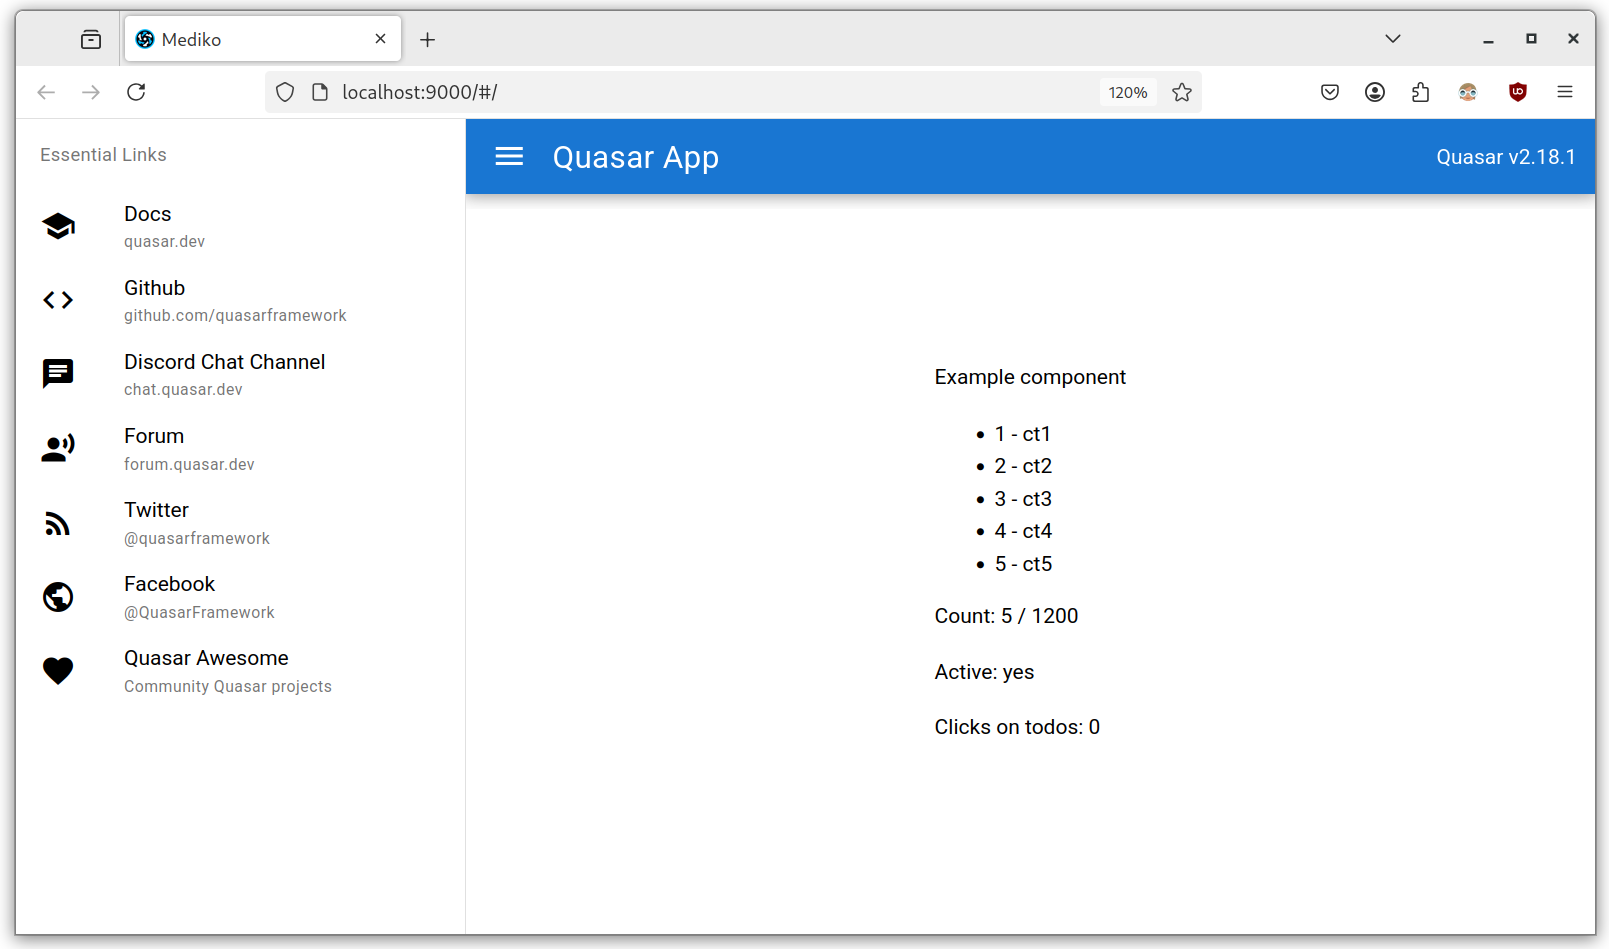
\includegraphics[width=0.8\textwidth]{templ-layout.png}
    \caption[Layout]{\label{fig:grail}Created Project template in web browser.}
\end{figure}


\section{\IfLanguageName{dutch}{Implementatie van de functionaliteiten}{Implementation of Functionalities}}%
\label{sec:functionalities}
% Logbooks, log, edit logs, 
% class diagram
% Local Storage


\section{\IfLanguageName{dutch}{Electron Desktop applicatie}{Electron Desktop Application}}%
\label{sec:desktop}
% Electron, VirtualBox

\section{\IfLanguageName{dutch}{Mobile Android}{Mobile Android}}%
\label{sec:mobile}
% Cordova, Android, Android Studio


\chapter{\IfLanguageName{dutch}{Gegevenssynchronisatie}{Data Synchronization}}%
\label{ch:synchronisation}
% nestjs, mysql, accounts